\documentclass[11pt]{article}

\author{Groep 6:\\
		Niels Desair\\
		Bram Kelchtermans\\
		Dylan Toirkens}
		
\title{\textbf{Studie van meetbare objectieven en ontwerpprincipes van Shneidermann}}

\date{19/10/2016}

\usepackage{graphicx}
\usepackage{parskip}
\usepackage{float}

\begin{document}
	\begin{titlepage}
		
		\newcommand{\HRule}{\rule{\linewidth}{0.5mm}} % Defines a new command for the horizontal lines, change thickness here
		
		\begin{center} % Center everything on the page
			
			\textsc{\LARGE Universiteit Hasselt}\\[1.5cm] % Nme of your university/college
			\textsc{\Large Humane en sociale aspecten van de informatica}\\[0.5cm] % Major heading such as course name
			
			\HRule \\[0.4cm]
			{ \huge \bfseries Studie van meetbare objectieven en ontwerpprincipes van Shneidermann}\\[0.4cm]
			\HRule \\[1.5cm]
			
			\begin{minipage}{0.4\textwidth}
				\begin{flushleft} \large
					\emph{Groep 6:}\\
					Niels \textsc{Desair} \newline
					Bram \textsc{Kelchtermans} \newline
					Dylan \textsc{Toirkens}
				\end{flushleft}
			\end{minipage}
			~
			\begin{minipage}{0.4\textwidth}
				\begin{flushright} \large
					\emph{Datum:}\\
					19 Oktober 2016
					\emph{Academiejaar: } \\
					2016-2017
				\end{flushright}
			\end{minipage}\\[4cm]
			\vspace{40 mm}
			\includegraphics[width=3.0cm]{uhasselt-logo}\\[2.0cm]  
		\end{center}
	\end{titlepage}

\section{Inleiding}
Voor het vak Humane en Sociale Aspecten van de Informatica is ons gevraagd om twee applicaties te vergelijken. Dit op het vlak van de ontwerpprincipes van Norman en op het vlak van metaforen. Deze paper zal bestaan uit drie individuele delen waarna we afsluiten met een gezamelijke conclusie. We hebben besloten om de communicatieapplicaties Skype en Google Hangouts te bespreken. We gebruiken de Google Hangouts extensie, dus niet de website.
\newpage

\section{Bespreking Niels}
Om een beter begrip te krijgen over hoe de User Interfaces (UIs) van beide applicaties tegen over elkaar staan en welke er eventueel beter is, ga ik ze vergelijken aan de hand van de ontwerpprincipes van Norman en zal ik enkele metaforen van beide programma's aanhalen en vergelijken. Zo hoop ik duidelijkheid te krijgen van wat deze programma's goed doen en waar ze nog in kunnen verbeteren.
\subsection{Ontwerpprincipes van Norman}
\subsubsection{Visibility}
Bij zowel Skype als Hangouts ziet de gebruiker over het algemeen altijd wat hij kan doen: een persoon selecteren om mee te chatten, een persoon bellen of zelfs een afbeelding of bijlage verzenden. Dit alles is zeer duidelijk zichtbaar met herkenbare icoontjes en het altijd aanwezig zijn van duidelijke tooltips, bij beide programma's (figuur \ref{fig:HTooltips}). Waar echter wel het verschil tussen beide programma's zit, is het aanmaken van groepen en het toevoegen van contacten. Toevoegen van contacten werkt bij beiden op dezelfde manier: men moet in een zoekveld gegevens van de gewenste persoon invullen en het programma zal deze persoon dan zoeken. Bij Hangouts staat er duidelijk als placeholder "Nieuw gesprek", terwijl dit bij Skype slechts "zoeken" is, wat het moeilijker maakt om als nieuwe gebruiker te vinden hoe men nieuwe contacten moet toevoegen. Het aanmaken van groepen gaat makkelijk en duidelijk in skype: er is een aparte button voor, die hangouts niet heeft (figuur \ref{fig:Sgroep}). Bij deze twee puntjes kunnen ze van elkaar leren, het zou natuurlijk ideaal zijn als beide programma's duidelijke knoppen heeft voor beide (toch wel belangrijke) functies.
\newpage
\begin{figure}
	\centering
	
\includegraphics[width=0.25\textwidth]{Niels_HTooltips.jpg}
	\caption{Voorbeeld van een duidelijke tooltip in Hangouts}
	\label{fig:HTooltips}
\end{figure}
\begin{figure}
	\centering
	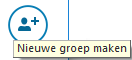
\includegraphics[width=0.25\textwidth]{Niels_groep.png}
	\caption{Knop met tooltip in Skype om een groep aan te maken}
	\label{fig:Sgroep}
\end{figure}
\subsubsection{Feedback}
Beide programma's geven uitstekende feedback. Denk maar aan het toevoegen van contacten (figuren \ref{fig:HContact} en \ref{fig:SContact}). Ook zijn er meerdere situaties waarin men feedback via meer dan 1 zintuig krijgt: wanneer men iemand belt, gebeld wordt, een bericht stuurt of krijgt of een contactverzoek binnenkrijgt, zal men bij zowel Skype als Hangouts een visuele feedback krijgen alsook een auditieve feedback, dit door een beltoon of berichttonen. Dit neemt de aandacht van de gebruiker en zal zeker de feedback duidelijk maken.
\begin{figure}
	\centering
	
\includegraphics[width=0.8\textwidth]{Niels_SkUitnodiging.png}
	\caption{Scherm na het verzenden van contactverzoek in Skype}
	\label{fig:SContact}
\end{figure}
\newpage
\begin{figure}
	\centering
	
\includegraphics[width=0.7\textwidth]{Niels_Uitnodiging.png}
	\caption{Scherm na het verzenden van contactverzoek in Hangouts}
	\label{fig:HContact}
\end{figure}
\subsubsection{Affordance}
Beide programma's maken gebruik van tal van affordances om de mogelijke acties die achter de buttons verschuild liggen duidelijk te maken. Hier kan men de verschillende bel knoppen in zowel Hangouts als Skype voor bekijken: er is een standaard telefoontje waarmee je kan bellen, alsook een video camera, waaruit duidelijk is dat dit bellen met video is (figuur
 \ref{fig:callicons}). Ook kan men afbeeldingen (Hangouts) of bijlagen in het algemeen (Skype) versturen, hiervoor is er naast het chatvenster telkens een duidelijk icoontje voorzien (figuren \ref{fig:afbeelding} en \ref{fig:bijlage}). Verder maken beide programma's hoofdzakelijk gebruik van toolbars en tekstmenu's, waardoor er weinig verwarring mogelijk is.
\begin{figure}
	\centering
	
\includegraphics[width=0.5\textwidth]{Niels_icoontjes.png}
	\caption{Knoppen voor video bellen en bellen bij Skype (links) en Hangouts (rechts)}
	\label{fig:callicons}
\end{figure}
\begin{figure}
	\centering
	
\includegraphics[width=0.1\textwidth]{Niels_afbeelding.png}
	\caption{Icoontje om een afbeelding te sturen in Hangouts}
	\label{fig:afbeelding}
\end{figure}
\begin{figure}
	\centering
	
\includegraphics[width=0.1\textwidth]{Niels_bijlage.png}
	\caption{Icoontje om een bijlage te sturen in Skype}
	\label{fig:bijlage}
\end{figure}
\newpage
\subsubsection{Mapping}
Bij Skype kan de grootte van het (input) chatvenster veranderd worden, hierbij verandert de cursor en ziet men duidelijk dat men naar boven (groter maken) en naar beneden (kleiner maken) kan bewegen, als men deze muisbewegingen doet, zal er gebeuren wat men verwacht (figuur \ref{fig:resize}). Dit ontbreekt volledig bij Hangouts en is dan ook een geldig punt van kritiek.

\begin{figure}
	\centering
	
\includegraphics[width=0.8\textwidth]{Niels_SResize.png}
	\caption{De cursor verandert wanneer men het chatvenster kan vergroten of verkleinen in Skype}
	\label{fig:resize}
\end{figure}
\subsubsection{Constraints}
Skype verhindert het starten van een gesprek wanneer dit niet kan, denk bijvoorbeeld aan een groepsgesprek met een lege groep. De buttons zullen dan meer transparant worden om duidelijk te maken dat deze onbeschikbaar zijn (figuur \ref{fig:skypeconstraint}). Verder zijn beide programma's zeer flexibel, ze hangen bijna volledig af van de interactie tussen gebruikers en hebben dan ook weinig constraints nodig, de gebruikers moeten de controle behouden.
\begin{figure}
	\centering
	\includegraphics[width=0.55\textwidth]{Niels_SConstraint.png}
	\caption{Uitgeschakelde bel buttons in een lege groep in Skype}
	\label{fig:skypeconstraint}
\end{figure}
\newpage
\subsection{Metaforen}
Beide programma's gebruiken dezelfde duidelijke 2 metaforen in dezelfde situatie: bij het bellen en bij het videobellen.
De brondomeinen zijn die van de videocamera en de mobiele telefoon. Dit zijn twee dingen waar de doorsnee gebruiker zeker ervaring me heeft, waardoor metaforen uit deze applicaties zeer bruikbaar zijn.
Als doeldomein hebben we het videobellen en het normaal bellen. De icoontjes hiervoor komen overeen met de brondomeinen, alsook de feedback: de beltonen, de notificaties, de camera, de mogelijkheid om berichtjes te sturen... Ze komen allemaal mooi overeen.
Echte mismatches zijn er niet - de vergelijkingen houden over het algemeen altijd stand. Uiteraard zijn zowel Skype als Hangouts meer uitgebreid in hun gebruik dan de standaard mobiele telefoon en videocamera.
\newpage

\section{Bespreking Bram}
\subsection{Ontwerpprincipes van Norman}
\subsubsection{Visibility}
Visibility wil zeggen dat alle mogelijke acties en opties meteen zichtbaar moeten zijn voor de gebruiker. Persoonlijk vind ik dat Google Hangouts op dit vlak verder staat dan Skype. Op Figuur \ref{fig:BeginHangouts} is het beginscherm van Hangouts te zien, meteen zijn ook alle functionaliteiten zichtbaar. Zo kan je een contactpersoon bellen, zoeken of toevoegen. Ook kan je zien welke gesprekken je de voorbije tijd gevoerd hebt en met wie. Een nadeel aan Skype is te zien op Figuur \ref{fig:BeginSkype}, zelf vind ik het zeer onduidelijk hoe men een contactpersoon moet zoeken of toevoegen. Wanneer men beter kijkt ziet men onder de eigen profielfoto een zoekvakje. In eerste instantie zou men denken dat dit enkel is om te zoeken, echter is dit ook bedoeld om contactpersonen toe te voegen. Persoonlijk vind ik dit zeker niet duidelijk voor een gebruiker die Skype niet kent. Wat dan wel in het voordeel van Skype speelt is het feit dat men kan kiezen tussen "contactpersonen" en "recent", dit terwijl bij Hangouts men vastzit aan "recent". Het is dus in Hangouts moeilijker om een overzichtelijke lijst van contacten te verkrijgen. Hangouts maakt dit dan wel goed door duidelijk een knop te voorzien om een nieuw gesprek te starten met (eventueel meerdere) contactpersonen.
\newline
De basisfuncties zoals bellen, chatten... zijn wel meteen en duidelijk zichtbaar in beide applicaties. De gebruiker selecteert of zoekt de gewenste contactpersoon en belt deze op met de daarvoor bestemde icoontjes. Deze icoontjes worden verder besproken in het deel "Affordance".
\begin{figure}
	\centering
	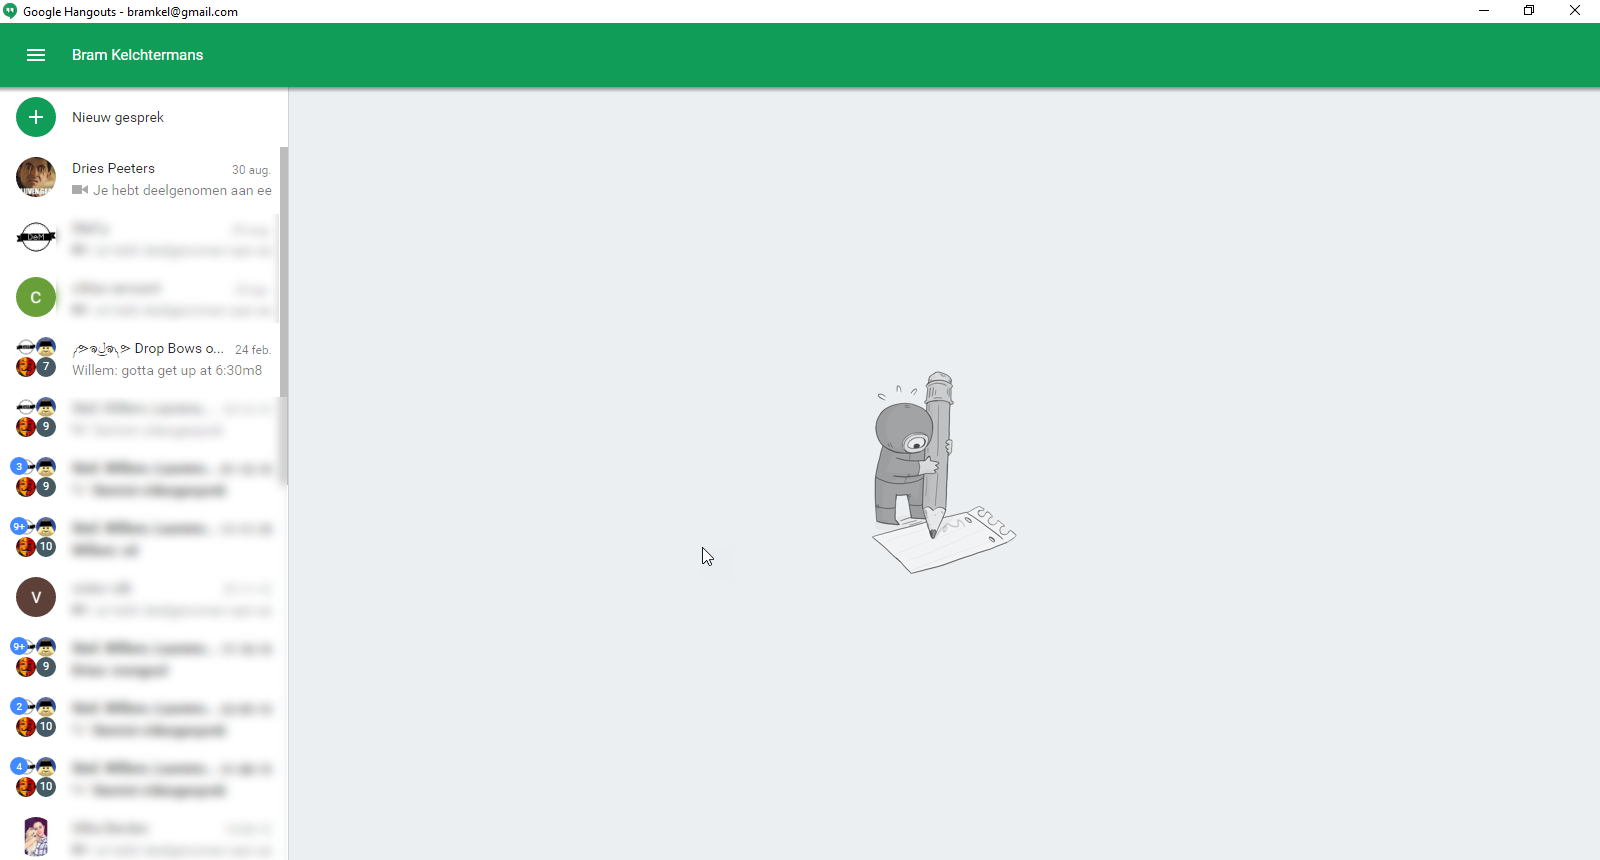
\includegraphics[width=1\textwidth]{Bram_ScreenshotGH1.png}
	\caption{Beginscherm van Hangouts}
	\label{fig:BeginHangouts}
\end{figure}
\begin{figure}
	\centering
	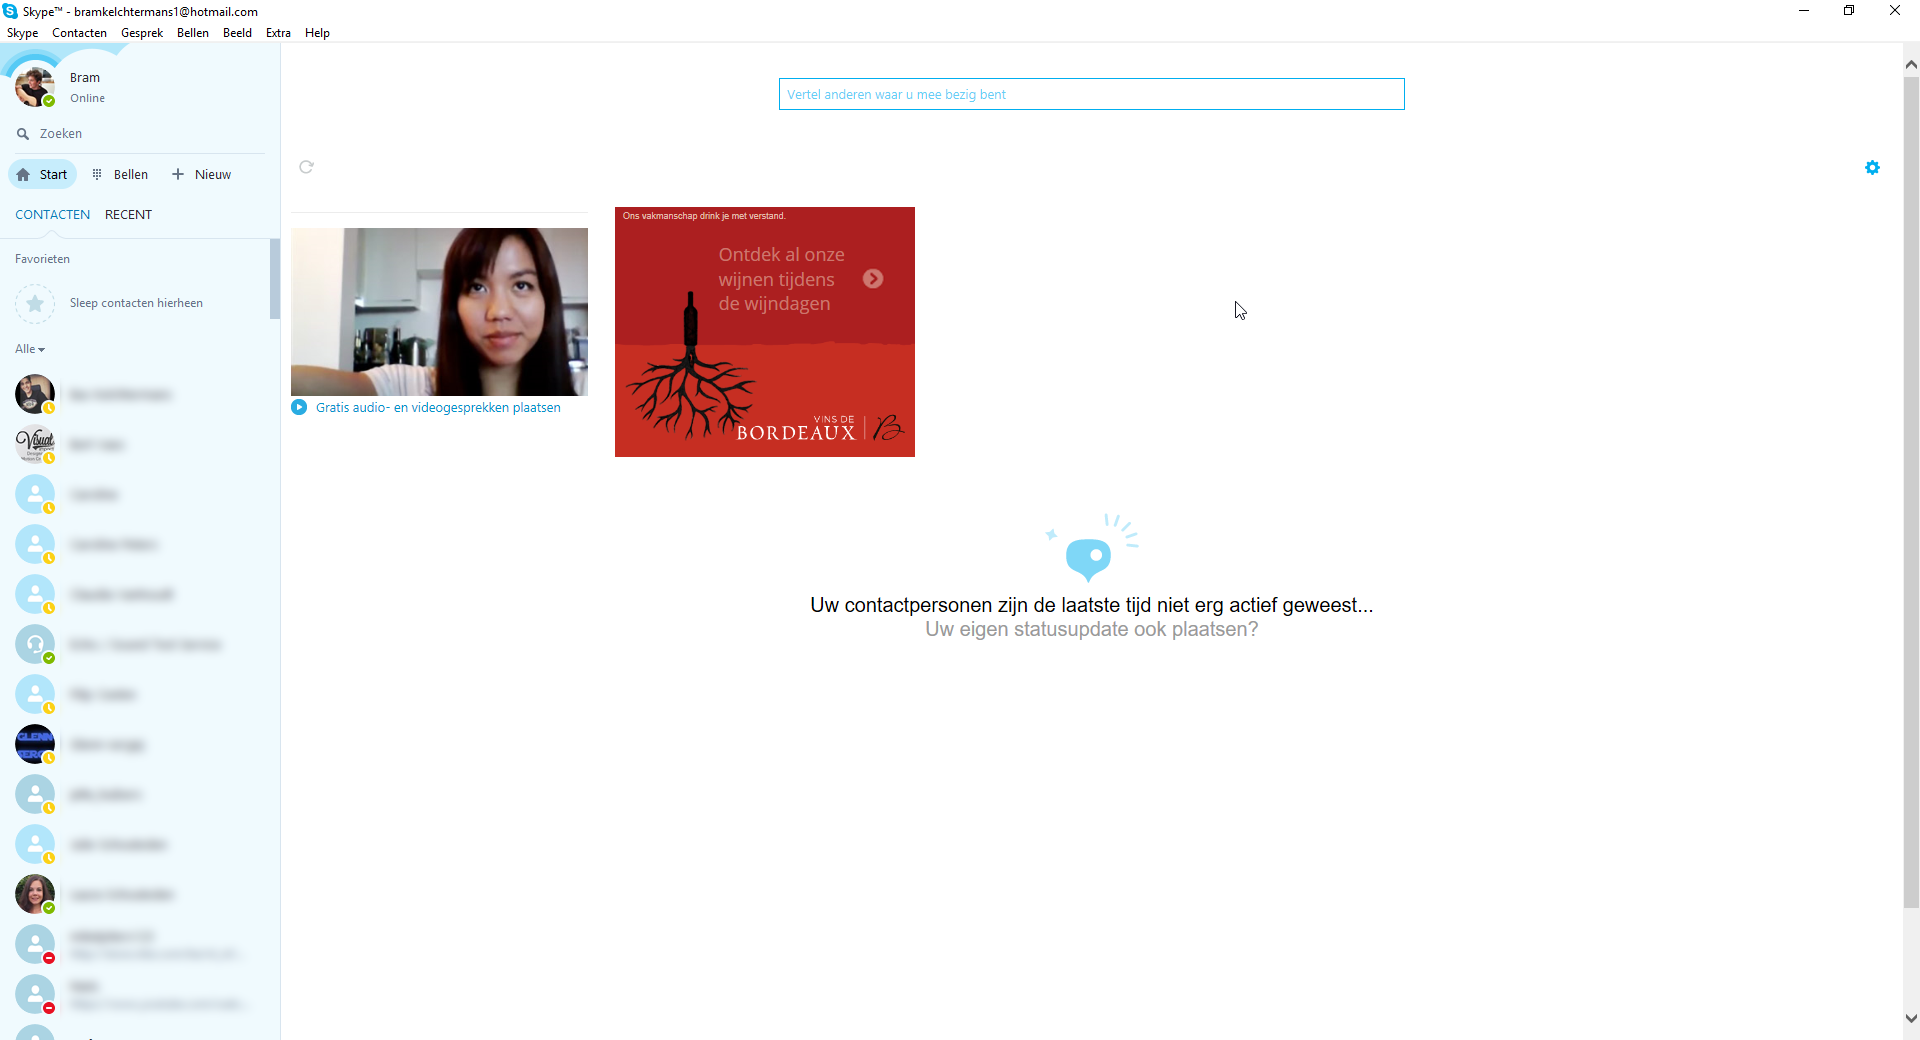
\includegraphics[width=1\textwidth]{Bram_ScreenshotSkype1.png}
	\caption{Beginscherm van Skype}
	\label{fig:BeginSkype}
\end{figure}
\subsubsection{Feedback}
Bij beide applicaties wordt er goed gebruik gemaakt van feedback. Dit vooral in de vorm van auditieve en tekstgebaseerde feedback. Zo wordt er telkens wanneer de gebruiker iemand belt een beltoon gespeeld, dit zodat de gebruiker weet dat de contactpersoon het verzoek om te bellen aan het ontvangen is. De ontvanger van de oproep hoort dan weer een beltoon op zijn of haar computer die aangeeft dat er iemand belt. Wanneer de contactpersoon echter niet bereikbaar is, krijgt de gebruiker duidelijk te horen dat de oproep niet beantwoord werd. Dit met een geluidstoon die duidelijk het einde van het gesprek aangeeft, ook krijgt de gebruiker een tekstgebaseerde feedback dat de contactpersoon niet bereikbaar is.
\newline
Een ander voorbeeld van feedback is te zien in figuur \ref{fig:VerzoekHangouts} voor Hangouts en in figuur \ref{fig:VerzoekSkype} voor Skype. In beide gevallen heeft de gebruiker een verzoek gestuurd om contactpersonen te worden met een persoon. Om te bevestigen dat de desbetreffende persoon een verzoek heeft ontvangen gebruiken beide applicaties een tekstboodschap als feedback. In beide applicaties wordt er in de chatsessie veel feedback gegeven. Zo ziet de gebruiker de volledige gespreksgeschiedenis met de geselecteerde contactpersoon. Dit gaat dan over gespreksduur, chatberichten...
\begin{figure}
	\centering
	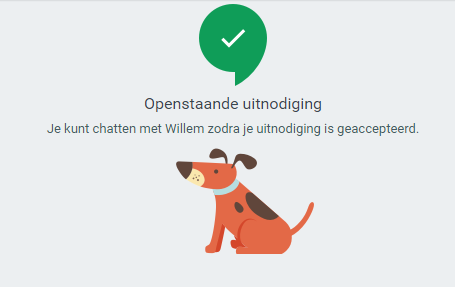
\includegraphics[width=0.7\textwidth]{Bram_ScreenshotGH2.png}
	\caption{Contactverzoek in Google Hangouts}
	\label{fig:VerzoekHangouts}
\end{figure}
\begin{figure}
	\centering
	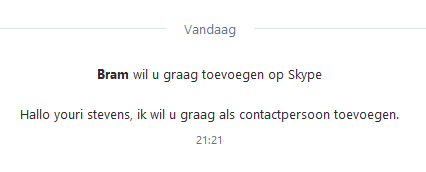
\includegraphics[width=0.7\textwidth]{Bram_ScreenshotSkype2.png}
	\caption{Contactverzoek in Skype}
	\label{fig:VerzoekSkype}
\end{figure}
\newline
Feedback is een zeer belangrijk aspect in deze context. Deze feedback is ook een soort metafoor aangezien de gebruiker dit kan mappen naar het brondomein: het telefoongesprek. In dit brondomein wordt er gebruik gemaakt van dezelfde soort auditieve feedback zoals de beltoon.
\subsubsection{Affordance}
Door het gebruik van metaforen en tekstgebaseerde GUI items is het snel duidelijk welke functie een bepaald element heeft. Zoals al eerder besproken heeft Skype een minpunt op dit vlak. Denk maar aan de zoekbalk van Skype, het is hier zeker niet duidelijk dat deze ook dient om nieuwe contacten te vinden. Bij Hangouts is dit echter wel duidelijk omdat er een grote knop met een "+" voorzien is, met de uitleg "Nieuw gesprek". Deze uitleg is belangrijker dan op het eerste zicht zou lijken, een nieuwe gebruiker zou bijvoorbeeld kunnen denken dat de knop enkel functie heeft om nieuwe contacten toe te voegen. 
\newline
Hangouts heeft echter ook een slechte affordance. Zoals te zien is in figuur \ref{fig:SoortHangouts} krijgt de gebruiker alleen de mogelijkheid om een videogesprek te starten. De gebruiker weet niet dat de camera tijdens het gesprek uitgeschakeld kan worden. Een nadeel is dus dat de gebruiker niet de mogelijkheid krijgt om een gesprek te starten zonder videobeelden.
\newline
 Verder is het wel duidelijk in beide applicaties hoe men een contactpersoon selecteert en deze dan kan contacteren. Ook is het duidelijk waar de gebruiker moet typen om een chatbericht achter te laten. 
 \subsubsection{Mapping}
 Bij het bellen via Skype of Hangouts kan je twee soorten gesprekken onderscheiden: spraakgesprekken of videogesprekken. Het is belangrijk dat de gebruiker duidelijk weet welk gesprek er gestart wordt. In figuur \ref{fig:SoortSkype} is de mapping duidelijk. De gebruiker krijgt de keuze welk soort gesprek er gestart zal worden. Deze mapping is ook van toepassing in Hangouts, hier wordt echter de nadruk gelegd op videogesprekken (zoals te zien is in figuur \ref{fig:SoortHangouts}).
 \begin{figure}
	\centering
	
\includegraphics[width=0.4\textwidth]{Bram_ScreenshotSkype3.png}
	\caption{Soorten gesprekken in Skype}
	\label{fig:SoortSkype}
\end{figure}
\begin{figure}
	\centering
	
\includegraphics[width=0.4\textwidth]{Bram_ScreenshotGH3.png}
	\caption{Soorten gesprekken in Hangouts}
	\label{fig:SoortHangouts}
\end{figure}
 \subsubsection{Constraints}
Beide applicaties hebben verschillende constraints. In Hangouts kan een gebruiker bijvoorbeeld niemand bellen die hem of haar niet geaccepteerd heeft als contactpersoon. Zo probeert Google te vermeiden dat er ongewenste gesprekken binnenkomen bij de gebruikers. Ook bij Skype is de mogelijkheid om een videogesprek te voeren met iemand die niet in de contactenlijst staat buiten werking gesteld. Het is echter wel nog mogelijk om een spraakgesprek te voeren met deze persoon. Persoonlijk vind ik dat Skype dit beter oplost, het kan zich namelijk voordoen dat je een persoon wilt contacteren die niet in je contactenlijst staat. Aangezien Skype deze mogelijkheid biedt in de vorm van een spraakgesprek is zeker een pluspunt.
\subsection{Metaforen}
Er zijn in beide applicaties duidelijke metaforen. Zo is het brondomein wel zeer duidelijk: het telefoongesprek. De icoontjes (zoals te zien in figuur \ref{fig:SoortSkype} en figuur \ref{fig:SoortHangouts}) maken duidelijk gebruik van de kennis van de gebruiker. Ook de geluiden zijn bekend voor de gebruiker, denk maar aan de wachttonen, beltonen... 
\newline
Als men als brondomein de mobiele telefoon neemt zijn er nog meer metaforen. Zo kan men tekst berichten versturen, zoals een SMS. Het versturen van een MMS is ook verwerkt in beide applicaties, de gebruiker kan namelijk foto's en video's versturen. 
\newline
Beide programma's hebben echter ook mismatches. Deze zijn echter bewust, denk zo aan de groepsgesprekken of de mogelijkheid om bestanden door te sturen. Deze functionaliteiten zorgen voor meer gebruiksgemak. 
\newline
Een recent toegevoegde functie aan beide applicaties is het achterlaten van een voicemail. Ook hier is een mismatch aanwezig aangezien de gebruiker ook een videobericht kan achterlaten voor de contactpersoon. Het spreekt voor zich dat dit niet het geval is bij een 'ouderwets' telefoongesprek.
\newpage

\section{Bespreking Dylan}
\subsection{Ontwerpprincipes van Norman}
\subsubsection{Visibility}
Wanneer je Skype of Hangouts voor het eerst gebruikt, dan vind ik op het eerste zicht dat Hangouts duidelijker laat zien hoe je een hoe je een gesprek met iemand kan starten. Dit omdat er onmiddelijk een functie te zien is om een nieuw gesprek te starten, waarna je dan een contactpersoon kan opzoeken (figuur \ref{fig:HNieuwGesprek}). In Skype is dit iets minder duidelijk. Om een contactpersoon toe te voegen, kan men dit doen via het menu, maar je kan ook onmiddelijk personen opzoeken via de zoekfunctie die te vinden is onder je profiel (figuur \ref{fig:SZoeken}). Ik vind echter dat deze zoekbalk niet duidelijk maakt dat ze gebruikt kan worden om zowel je eigen contactenlijst te doorzoeken of om nieuwe contacten te zoeken. Op het eerste zicht zou ik enkel denken dat het dient om personen in je eigen contactenlijst te vinden. Dit is dus een minpunt van Skype. Toch biedt Skype hier een oplossing voor bij nieuwe gebruikers. Nadat je een nieuw account hebt aangemaakt, krijg je een berichtje van Skype met een aantal links naar tutorials en vragen (figuur \ref{fig:STips}). Hiermee probeert Skype nieuwe gebruikers vanaf het begin al op weg te helpen. Wat bij beide applicaties wel goed zichtbaar is, zijn de mogelijke functionaliteiten bij het chatten en bellen. De plaats waar je je bericht kan ingeven en de icoontjes om een videogesprek te starten, emoticons in te voegen of een bestand door te sturen zijn makkelijk terug te vinden. 
 \begin{figure}
	\centering
	
\includegraphics[width=0.9\textwidth]{Dylan_HNieuwGesprek.png}
	\caption{Een gesprek starten in Hangouts}
	\label{fig:HNieuwGesprek}
\end{figure}
\begin{figure}
	\centering
	
\includegraphics[width=0.4\textwidth]{Dylan_SZoeken.png}
	\caption{Personen zoeken en toevoegen in Skype kan via de zoekbalk}
	\label{fig:SZoeken}
\end{figure}
\begin{figure}
	\centering
	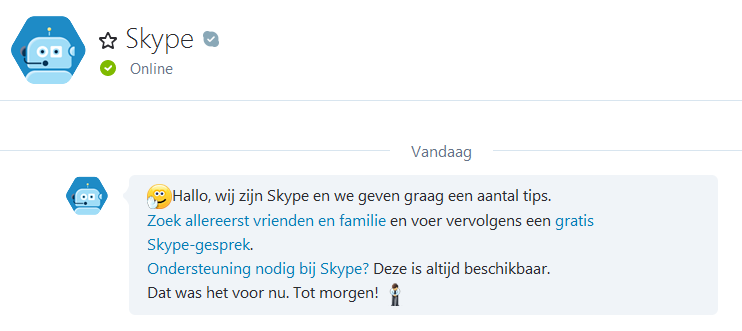
\includegraphics[width=0.9\textwidth]{Dylan_STips.png}
	\caption{Nieuwe gebruikers krijgen tips van Skype}
	\label{fig:STips}
\end{figure}
\subsubsection{Feedback}
In beide programma's is er duidelijke feedback voorzien. Zo is er bijvoorbeeld een specifiek geluid wanneer je een nieuw bericht ontvangt of wanneer je gebeld wordt. Naast auditieve feedback is er ook veel visuele feedback, meestal in de vorm van een klein tekstje. Skype laat bijvoorbeeld niet alleen zien wanneer een oproep mislukt is, maar verteld hierbij ook de reden waarom het niet gelukt is. (figuur \ref{fig:SFeedbackGesprek}). Na een videogesprek toont Skype hoelang een gesprek heeft geduurt, terwijl Hangouts meldt wie er deelgenomen heeft aan het gesprek. Een ander puntje waar beide programma's feedback leveren is bij het starten van een gesprek met een nieuwe contactpersoon. In beide programma's wordt eerst gevraagd om een verzoek te sturen om elkaar als contactpersoon te hebben. De verzender krijgt een bericht dat het verzoek verzonden is, terwijl de onvanger deze kan bevestigen of weigeren. Er wordt ook feedback geleverd op de online status van anderen. In Hangouts toont een groen bolletje of iemand online is (figuur \ref{fig:HOnline}), maar je kan je eigen status niet aanpassen. In Skype zijn er verschillende icoontjes die de status weergeven en je eigen status is ook weergegeven bij je profiel (figuur \ref{fig:SStatus}).
\begin{figure}
	\centering
	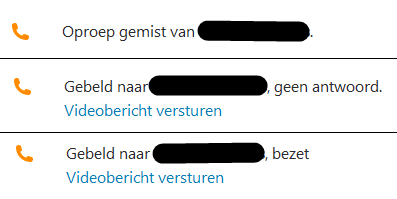
\includegraphics[width=0.4\textwidth]{Dylan_SFeedbackGesprek.png}
	\caption{Skype laat weten waarom een gesprek niet is gelukt}
	\label{fig:SFeedbackGesprek}
\end{figure}
\begin{figure}
	\centering
	
\includegraphics[width=0.1\textwidth]{Dylan_HOnline.png}
	\caption{Het groene bolletje in Hangouts meldt dat de persoon online is}
	\label{fig:HOnline}
\end{figure}
\begin{figure}
	\centering
	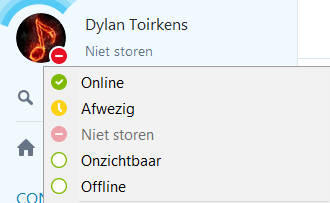
\includegraphics[width=0.4\textwidth]{Dylan_SStatus.png}
	\caption{De verschillende online statussen in Skype}
	\label{fig:SStatus}
\end{figure}
\subsubsection{Affordance}
De meeste icoontjes in beide programma's hebben een duidelijke functie. Dit omdat ze overeenkomen met heel wat andere applicaties. De symbolen om te bellen, bestanden door te sturen en emoticons in te voegen zijn snel herkenbaar (figuur \ref{fig:SHIcoontjes}). Zoals eerder aangehaald, is de zoekfunctie van Skype een stuk minder duidelijk (figuur \ref{fig:SZoeken}). Het is nl. niet duidelijk dat deze ook gebruikt kan worden om nieuwe personen toe te voegen. 
\begin{figure}
	\centering
	
\includegraphics[width=0.4\textwidth]{Dylan_SHIcoontjes.png}
	\caption{De icoontjes in Skype (links) en Hangouts (rechts) zijn zeer herkenbaar}
	\label{fig:SHIcoontjes}
\end{figure}
\subsubsection{Mapping}
Wanneer je chat met meerdere mensen, zou het handig zijn om te weten wie wat stuurt (en ook welke berichten je zelf hebt gestuurd). Beide programma's tonen een tekstballon met een pijltje naar recht voor berichten die je zelf hebt gestuurd. Bij alle andere personen staat het pijltje naar links gericht. Daarnaast wordt er ook enkel bij berichten van anderen ook de naam en de profielfoto weergegeven naast de tekstballon (figuur \ref{fig:HChat}).
\begin{figure}
	\centering
	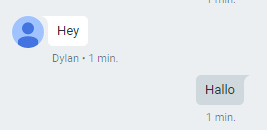
\includegraphics[width=0.4\textwidth]{Dylan_HChat.png}
	\caption{De tekstballonen maken duidelijk wie een bericht gestuurd heeft}
	\label{fig:HChat}
\end{figure}
\subsubsection{Constraints}
Er zijn verschillende constraints in beide programma's. Zo is het bijvoorbeeld niet mogelijk zijn om een bericht te sturen met enkel spaties. De bedoeling hiervan is dat er geen "leeg bericht" verstuurd kan worden. Ook worden bepaalde knoppen uitgeschakeld wanneer ze niet gebruikt kunnen worden, zoals een videogesprek starten terwijl niemand anders in de groep zit.
\subsection{Metaforen}
In beide programma's zijn de metaforen duidelijk te zien. Ze worden allebei gebruikt wanneer je berichten stuurt of belt naar iemand via Skype of Hangouts. De brondomeinen zijn een (mobiele) telefoon en een videocamera. Als we naar de icoontjes kijken die in deze context gebruikt worden, kunnen we hun functionaliteit snel afleiden. De knop om een gesprek te be\"eindigen  komt overeen met het ophangen van een telefoon. De knop met een camera en die met een microfoon laten weten of respectievelijk de camera en microfoon aan- of uitstaan (figuur \ref{fig:SHMetafoor}). Ook de geluiden die afgespeeld worden zijn goed te vergelijken met een telefoongesprek. Er zijn echter niet veel mismatches. Een voorbeeld hiervan is de mogelijkheid om in Skype naast foto's en video's ook bestanden door te sturen. In Hangouts is het niet mogelijk om bestanden door te sturen. Toch hebben beide programma's meer funcionaliteiten dan een camera en een telefoon. Het is bijvoorbeeld mogelijk om je scherm te delen tijdens een videogesprek. Deze extra functies zijn voornamelijk bedoeld om het gebruiksgemak te bevorderen en de gebruiker extra mogelijkheden te bieden.
\begin{figure}
	\centering
	
\includegraphics[width=0.4\textwidth]{Dylan_SHMetafoor.png}
	\caption{Icoontjes voor microfoon, gesprek be\"eindigen en camera van Hangouts (boven) en Skype (onder)}
	\label{fig:SHMetafoor}
\end{figure}
\newpage


\section{Gezamelijnke Conclusie}
\subsection{Inleiding}
Nu we elk onze eigen inbreng hebben gegeven gaan we onze verschillende standpunten samenbrengen in deze conclusie. In deze paragraaf wordt dezelfde structuur behouden en dus zullen we het hier hebben over de ontwerpprincipes van Norman waarna we vervolgen met een stuk over metaforen.

\subsection{Ontwerpprincipes van Norman}
\subsubsection{Visibility}
Over het algemeen zijn we het eens dat de basisfuncties van de programma's duidelijk zichtbaar zijn voor de gebruiker. We zijn het er ook over eens dat beide applicaties kunnen leren van elkaar. Samen zijn we tot de conclusie gekomen dat de zoek- en toevoegfunctie van Skype te wensen overlaat. Het is hier niet duidelijk dat deze zoekbalk ook de functionaliteit van toevoegen bevat. Dylan wijst wel op een positief punt van Skype. Wanneer een gebruiker namelijk een nieuw account aanmaakt zal deze verschillende tutorials ter beschikking krijgen die meteen worden meegedeeld. Hangouts heeft deze tutorials ook, maar de gebruiker zal deze zelf moeten zoeken. \newline Wat ook in het voordeel van Skype speelt, is de onderverdeling van contactpersonen. Bram haalt namelijk aan dat de gebruiker een mogelijkheid krijgt om te navigeren door de contacten. Zo is er de mogelijkheid om een lijst te krijgen van de contacten, waar meteen zichtbaar is welke contacten online zijn. Een tweede mogelijkheid zit in het tablad "Recent" (Figuur \ref{fig:SkypeTabblad}), hier krijgt de gebruiker de mogelijkheid om een overzicht te krijgen van de meest recent gevoerde conversaties. In Hangouts wordt enkel de mogelijkheid gegeven om de recente gesprekken weer te geven, dit kan voor verschillende gebruikers verwarrend en dus een minpunt zijn.
\begin{figure}
	\centering
	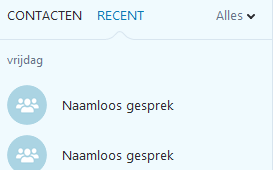
\includegraphics[width=0.4\textwidth]{Samen_SkypeTabblad.png}
	\caption{Onderverdeling contactpersonen in Skype}
	\label{fig:SkypeTabblad}
\end{figure}
\newline
Zoals al eerder besproken heeft Hangouts ook wel een stap voor op Skype. Daarmee bedoelen we dat Hangouts een duidelijker element heeft om contactpersonen te zoeken of toe te voegen. Dit is te zien in de placeholder op figuur \ref{fig:HangoutsNew}. Dit is zeker een groot pluspunt aan Hangouts.
\newline
We kunnen dus zeggen dat op het vlak van visibility beide applicaties nog wat aanpassingen kunnen verrichten. Ze kunnen hier echter op verschillende vlakken wel een voorbeeld nemen aan elkaar.
\begin{figure}
	\centering
	
\includegraphics[width=0.4\textwidth]{Samen_HangoutsNew.png}
	\caption{Zoeken en toevoegen van contacten in Hangouts}
	\label{fig:HangoutsNew}
\end{figure}
\subsubsection{Feedback}
Bij applicaties zoals Skype en Hangouts is feedback een belangrijk aspect om te bespreken. De gebruiker moet namelijk weten of de uitgevoerde acties daadwerkelijk effect hebben. We denken dan niet alleen aan het opbellen van personen maar ook aan het toevoegen van contacten. 
\newline
Beide applicaties hebben hier goed werk verricht. Er zijn namelijk verschillende vormen van feedback die de gebruiker helpen. Zo is er tekstgebasseerde en auditieve feedback.
\newline
Een voorbeeld van tekstgebasseerde feedback is te zien in figuur \ref{fig:VerzoekHangouts} en figuur \ref{fig:VerzoekSkype}. De gebruiker heeft in beide applicaties een contactverzoek gestuurd. Beide applicaties laten aan de gebruiker weten dat het verzoek succesvol is verzonden en dat de gebruiker moet wachten op een acceptatie. Een andere voorbeeld van tekstgebasseerde feedback is de gespreksgeschiedenis die te zien is in het chatvenster. Zo kan de gebruiker zien wanneer hij of zij een gesprek gevoerd heeft en voor hoe lang. Dylan haalt in zijn deel ook aan dat de gebruiker feedback krijgt wanneer een oproep mislukt is. Dit is te zien in figuur \ref{fig:SFeedbackGesprek}. Deze feedback geeft aan dat het gesprek mislukt is, alsook de reden waarom dit gesprek niet gelukt is.
\newline
Een andere belangrijke vorm van feedback is de auditieve feedback. Het is namelijk zeer belangrijk dat de gebruiker weet wanneer hij of zij wordt opgebeld of zelf iemand aan het bellen is. Dit wordt in beide applicaties voorzien door een beltoon die afgespeeld wordt in de verschillende situaties. Er worden ook verschillende beltonen gebruikt voor het opbellen en het opgebeld worden. Dit is zeker belangrijk aangezien de gebruiker zo duidelijk weet waarmee hij of zij bezig is. 
\newline
Dylan bespreekt nog een andere soort feedback. Namelijk de status van de contactpersoon, denk zo bijvoorbeeld aan "Online", "Afwezig", "Bezet"... Deze feedback is van groot belang aangezien de gebruiker zo weet welke contactpersonen bereikbaar zijn en welke eventueel het gesprek niet zullen opnemen. Skype heeft hier echter wel meer mogelijkheden. Hangouts heeft namelijk maar twee statussen: "Online" of "Offline", deze status wordt tevens automatisch aangepast zonder de inbreng van de gebruiker. 
\subsubsection{Affordance} 
Over het algemeen zijn we het er over eens dat de verschillende UI elementen een duidelijke functie hebben. Dit doordat de gebruikte symbolen en iconen vanzelfsprekend zijn en toespraak doen op de kennis van de gebruiker. Dit wordt nog uitgebreid besproken in het deel "Metaforen". 
\newline
Nochtans zijn er ook slechte affordances, we denken zo aan de zoekbalk van Skype. Zoals al eerder besproken is het voor de gebruiker niet duidelijk dat deze ook de mogelijkheid biedt om contactpersonen toe te voegen. Hangouts heeft hier een betere oplossing voor gevonden met de placeholder die hierboven besproken is en te zien is in figuur \ref{fig:HangoutsNew}.
\newline
Ook Hangouts heeft een slechte affordance zoals Bram al aanhaalt. Zoals te zien is in figuur \ref{fig:SoortHangouts} krijgt de gebruiker alleen de mogelijkheid om een videogesprek te starten. Wat de gebruiker echter niet weet is dat in de loop van het gesprek de camera ook gedeactiveerd kan worden. Aangezien de gebruiker geen mogelijkheid heeft om een audiogesprek te voeren, kunnen we zeggen dat dit een slechte affordance is. 
\newline  
Niels bespreekt ook nog de verschillende icoontjes die aanwezig zijn bij het chatvenster. We spreken dan over de icoontjes om bijlagen te versturen of een emoticon toe te voegen aan het chatbericht. Deze icoontjes zijn meteen duidelijk voor de gebruiker, dit doordat de icoontjes veel gebruikt worden en universeel zijn over verschillende applicaties.
\subsubsection{Mapping}
Tussen beide programma's zijn er voor dit principe niet veel verschillen te vinden. Wanneer bijvoorbeeld het input bericht groter wordt dan de ruimte waar het bericht ingegeven kan worden, zullen zowel Skype als Hangouts deze ruimte vergroten. Dit is echter beperkt tot een aantal regels, waarna er dan gewerkt wordt met een schuifbalk, zoals te zien is in figuur \ref{fig:SkypeGrootChatvenster}. Niels haalt wel aan dat een gebruiker de mogelijkheid heeft om de grootte van het chatvenster in Skype aan te passen. In figuur \ref{fig:resize} is te zien dat dit venster via de muis vergroot en verkleind kan worden. Hiermee kan een minimumgrootte bepaald worden. Deze functie is echter niet beschikbaar in Hangouts. 
\newline
In het deel "Affordance" hadden we al besproken dat het in Hangouts enkel mogelijk is om een videogesprek te starten. Skype biedt hier 2 verschillende knoppen voor, zodat de gebruiker kan kiezen tussen een videogesprek of een audiogesprek (figuur \ref{fig:SoortSkype}). Zoals eerder vermeld is dit een minpunt van Hangouts.
\newline
De tekstballonnen tijdens het chatten vormen een duidelijk voorbeeld van dit principe. In figuur \ref{fig:HChat} is te zien dat de richting van de tekstballonnen duidelijk maakt van wie een bericht is. Als ze naar rechts gericht zijn, is het een bericht dat de gebruiker zelf gestuurd heeft. Als ze naar links gericht zijn, dan is het een bericht van een andere gebruiker. Bij berichten van andere gebruikers wordt ook nog de naam en profielfoto getoond, wat zeker in het voordeel speelt wanneer er een gesprek gevoerd wordt met meerdere personen.
\begin{figure}
	\centering
	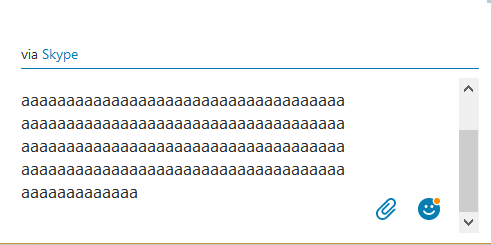
\includegraphics[width=0.6\textwidth]{Samen_SkypeGrootChatvenster.png}
	\caption{Een groot chatvenster met schuifbalk in Skype bij een groot input bericht}
	\label{fig:SkypeGrootChatvenster}
\end{figure}
\subsubsection{Constraints}
In programma's zoals Skype en Hangouts is het belangrijk om voldoende constraints te hebben, maar toch een zekere mate van flexibiliteit te houden. Dit houdt in dat gebruikers geen functies kunnen oproepen wanneer ze zinloos of ongewenst zijn. Een gebruiker kan bijvoorbeeld geen videogesprek starten in een lege groep of een bericht sturen met enkel spaties.
\newline
Bram bespreekt in zijn deel dat het in beide programma's niet mogelijk is om een videogesprek te voeren met iemand wanneer ze elkaar nog niet geacctepteerd hebben als contactpersoon. In deze situatie is het in Skype echter wel mogelijk om een spraakoproep met elkaar te hebben. Het aanbieden van deze mogelijkheid is dus zeker een pluspunt van Skype.
\subsection{Metaforen}
We zijn het eens met elkaar dat deze programma's een duidelijk metafoor hebben, met als brondomeinen het gebruik van een (mobiele) telefoon bij het sturen van berichten en het bellen, en een camera. De icoontjes voor het bellen zijn zeker bekend bij de gebruikers, ze representeren namelijk het opnemen en het ophangen van een telefoon. Bij een videogesprek zijn er ook knoppen om microfoon of camera uit te schakelen, zoals te zien is in figuur \ref{fig:SHMetafoor}. Daarnaast wordt er ook gebruik gemaakt van de herkenbare geluiden die afgespeeld worden bij het bellen. Zo is er bijvoorbeeld een ringtone wanneer een gebruiker gebeld wordt, en een geluid dat afspeelt wanneer de ontvanger nog niet opgenomen heeft. 
\newline
Bij het sturen van berichten kunnen we ook hier als brondomein een mobiele telefoon nemen. Een standaard tekstbericht komt overeen met een SMS, terwijl het verzenden van foto's en video's vergeleken kan worden met het sturen van een MMS.
\newline
Er zijn ook een aantal mismatches. Zo is het bijvoorbeeld mogelijk om groepsgesprekken te voeren met andere gebruikers. Bram bespreekt in zijn deel dat een recent toegevoegde functie de mogelijkheid biedt om een voicemail achter te laten. In tegenstelling tot een telefoon, kan er in beide applicaties ook een videobericht gestuurd worden. Dit is zeker een uitbreiding t.o.v. een voicemail via telefoon.
\newline
Een andere mismatch werd vermeld door Dylan. In het geval van MMS is het enkel mogelijk om foto's en video's te versturen. In Skype is het ook mogelijk om bestanden te verzenden naar andere gebruikers. Deze functie is echter niet mogelijk in Hangouts, waardoor ze dus meer een traditionele betekenis geeft aan een MMS. Toch is het versturen van bestanden zeker een handige optie, wat ds in het voordeel speelt van Skype. 
\newpage
\end{document}